%===================================== CHAP 3 =================================

\chapter{Implementation}

\textit{Detailed description of the web interface and its structure as well as case study, this was missing from the specialization project. \\
\noindent Present the technology used (might have to reword the name of this chapter). \\
\noindent Include several typical software development diagrams.}

\section{Visualization Tool}

\subsection{Prototype}

This section will describe the prototype of the web interface to be improved as well as some pointers on what should be implemented in the next version.

\subsubsection{Description}

\noindent The prototype provides all the basic user functionality for creating a user, and logging in and out, including validation of user name and password. A user can upload Python scripts from their computer to the server, and tag them with various topics to make them easier to search for, using the search bar on the page showing all uploaded scripts. \\

\noindent By selecting a specific script, the user can view the code, add tags to, delete, and of course run, the script. A separate menu tab for visualizations provides the user with visualizations of the data produced while running. The only visualization techniques implemented are the training progress and layer activations laid out after each other on a single page. The training progress includes two separate plots showing accuracy and loss over batch, while the layer activations are shown for each single layer of the network defined in the script.

\subsubsection{Planned Improvements}

The overall purpose will be to add more functionality with the goal of improving the user's understanding of the network. This may be new visualization techniques, training process statistics, better presentations of data, and more user controls. Another useful addition can be allowing the user more flexibility and make the visualizations more interactive.

\subsection{System Development Methodology}

The development of the visualization tool has been carried out by a team consisting of the two of us, with no specific set of roles. Because of the small team size, we did not see the need for a dedicated project manager. Both of us were involved in designing the architecture and interface, as well as implementing and testing the system, giving us great knowledge of the whole system. Still, we maintained an efficient workflow by dividing the programming task into two main responsibility areas, one for each of us:
\begin{enumerate}
    \item Visualizing data using the selected visualization library and incorporating these into the user interface
    \item Implementing visualization techniques and creating networks to illustrate the use of the tool with the chosen deep learning library
\end{enumerate}

\noindent The development process itself did not follow any strict guidelines, but included several elements from Agile methods. It has been an iterative and incremental process, starting with the existing prototype of the system that only implemented two of the visualization techniques in a very simple manner. Based on our own testing as well as feedback from the customer, which in this case is our supervisors, functionality were added and adjustments were made in order to obtain a new and improved prototype. This process was repeated until we reached a satisfactory system according to the initial requirements. An example of the iterative part of the process is when we decided to replace the old visualization library with a new one that better suited our needs. An example of the incremental part of the process is when our supervisors expressed the wish for a way for the user to be able to upload an image to be used in producing some of the visualizations. Other concepts from Agile development that were put into use are code review, pair programming, and the use of a backlog to get an overview of the requirements.

\subsection{Focus Quality Attributes}

\subsubsection{Modifiability}

An important aspect of the system design of the visualization tool is to make sure that any part can be easily replaced. For instance, it should not be too difficult to alter the system to use a different deep learning library than the one employed in our implementation. This requires thorough consideration when designing the architecture, and typically calls for a module-based architecture with each module being loosely coupled, meaning that it should interact with as few of the other modules as possible.

\subsubsection{Usability}

Not only should the interface be simple and easy to navigate for the user, but the actual installation of the program and the adaption of the user's deep learning scripts to the tool, should be without much trouble. A thorough user manual and documentation of the API is the key to obtaining this kind of usability. Preferably, we would want any ANN to run in our program without problems, but it is near to impossible to generalize this much. The main goal was thus to support the most commonly used networks, but at the same time, as the previous section mentions, easily allow for extending the system to work with different kinds of ANNs.

\subsection{Technology Decisions}

\subsubsection{Flask}

Flask is a web framework written in Python, used to build simple web applications. It is a micro-framework, meaning that it has very few dependencies to external libraries. It provides you with only the basic tools needed to create a web application, and is therefore very lightweight. There exists many plugins that can be added for an increased range of functionality. Since the focus of our visualization tool is not the web page itself, but rather its capabilities in terms of visualization techniques, Flask is the perfect choice. It allowed us to quickly set up an application and implement a basic user system and upload functionality.

\subsubsection{SQLite}

Very lightweight and easy to include in simple desktop apps that could make use of a database. Do not really need to store much data. Simple relational data. Not an important part of the application. Lightweight. Not a lot of connections.

\subsubsection{Keras}

Keras is a high-level neural networks library that can run on top of either TensorFlow or Theano. Its purpose is to provide a way to quickly and easily create models and start experimenting. It is very minimalistic, providing only enough to achieve an outcome, while still allowing for extensibility by making it easy to add and use new modules within the framework. Keras provides the user with several callbacks, i.e. sets of functions to be applied at giving stages of the ANN training procedure. It also allows for creating your own custom callbacks, which is perfect for our use case, since we then can create callbacks that produces the data needed for each visualization technique.

\subsubsection{TensorFlow}

Not sure if we need this section. But mention in Keras section, and say whether we support both Theano and TensorFlow?

\subsubsection{Bokeh}

Bokeh is a Python interactive visualization library for modern web browsers. It can easily be embedded into a Flask application, as we will show in a later section. The library is easy to use, and has the flexibility of adding interactions and highly advanced customization. Another benefit is that it is easy to stream large data sets and plot them live. \textit{Something about the drawbacks because it is new.}

A lot of possibilities for adding interactions, easy to stream live plotting of data. Drawbacks are that it is fairly new and still under development. Also probably not the best for handling images.

\subsection{Overview of the Architecture}

As seen in \textbf{Fig. \ref{architecture1}}, the system can be said to consist of five separate modules: Flask, Bokeh, Keras, the user storage and the database. The Flask module is the very core of the application, that defines the routes (URLs), models and forms of the web page, tying it all together with the HTML templates, CSS and JavaScript.

% First, the overall architecture. Explain the different modules.
% Then we can focus on some parts of the architecture that we want to "show off".

\begin{figure}[h!]
    \centering
        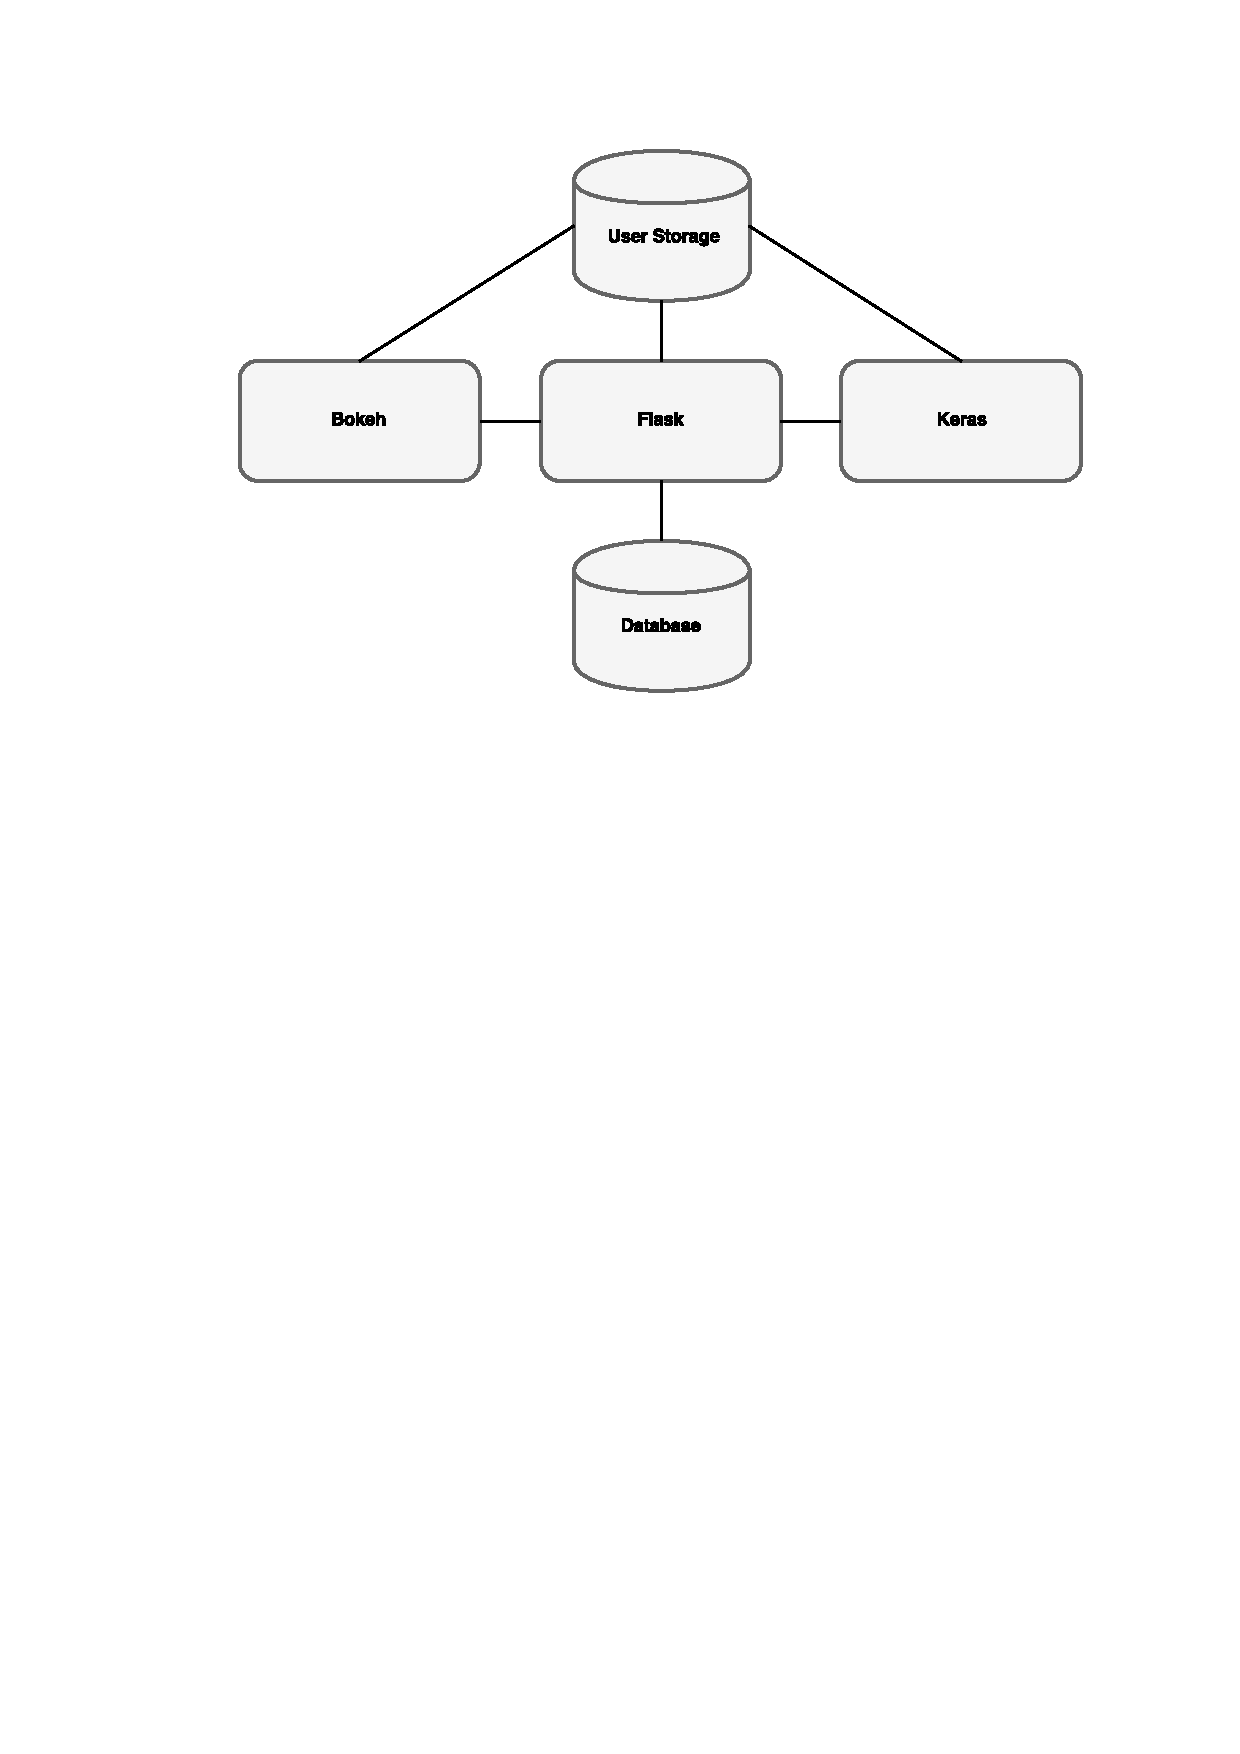
\includegraphics[width=1\textwidth]{fig/overall-architecture.pdf}
        \caption{Overall Architecture of the System}
        \label{architecture1}
\end{figure}

% Examples here are the relation between bokeh and flask, flask and keras, flask and the user storage. etc.

\subsection{The Flask Application}

\subsection{Spotlight2}

\subsection{Callbacks}
% Just say something about HOW the visualizations are implemented.
% We can refer the reader to an Appendix on exactly how to use them and what they are.

\subsection{Visualizations}

\subsection{Spotlight4}

\section{Case Study in Face Recognition}

\textit{Describe the case study (facial recognition with expression).
Should already be presented, but here we can add specifics, and also possibly describe the structure of the network we have created, the dataset used, etc.}


\cleardoublepage